% Interaction between DCS and DAQ
%FIXME this section is now a bit out of date

Close interaction between the DAQ and DCS (Detector Control System)
software systems are needed for the powering of the FPix, and also so
that special settings can be applied to the ROCs in case the high voltage is off.

From the DAQ side, the startup procedure is embedded
within the ``Initializing'' and ``Configuring'' FSM transitions
prescribed by Run Control. In working through these states, the DAQ
system must use information from the DCS system about the voltages being
applied across various detector and front-end elements. 

The XDAQ Supervisor applications mainly involved with this are:

\begin{itemize}
\item PixelFECSupervisor: Controls a crate of Pixel FEC boards
\item PixelTKFECSupervisor: Controls a crate of Tracker FEC boards
\item PixelDCSFSMInterface: Reports the voltages applied by the DCS 
      system (simplified to LV\_OFF/ LV\_ON\_REDUCED/ LV\_ON for low voltage
and HV\_OFF / HV\_ON for high voltage).
\end{itemize}

\subsection{PSX Server}
The gateway between DCS and our xdaq applications is the PSX
server. This server is a xdaq application that runs on the machine
{\tt cmspsx} at P5. This machine runs independent PSX server applications
for all of the different subdetectors. Both the machine and the
software running on it are administered by the central DAQ experts.

We interact with two separate PSX server application -- the ``Pixel
PSX server'' running on port 9923, and the ``Tracker PSX server''
running on port 9922. The Pixel PSX server is used for making
connections to DCS to learn the status of the power supplies (the
topic of this section). The Tracker PSX server is used to send DCU
data to DCS. Note that the Tracker PSX server is also used by the
strip tracker, and for performance reasons it has proven critical to
use the independent Pixel PSX server for making the connections to the
power supply status.

\subsection{PixelDCSFSMInterface}

The PixelDCSFSMInterface provides an interface between the PSX server and our other pixel xdaq applications. Changes in the states of each power supply modules are sent in real time from the PSX server to the PixelDCSFSMInterface application. The PixelDCSFSMInterface summarizes this information into one state per half cylinder/shell (thus there are 8 summarized states, 4 in the FPix and 4 in the BPix). The logic for making the summary is as follows:

\begin{itemize}
\item If all A4603 power supplies in the summary group are ON (HV and LV is ON), then the summarized state reflects this
	\begin{itemize}
	\item A4603 power supplies in state {\tt HVMIXED} (one HV channel is on and the other is either off or ramping), are treated as if they were ON.\footnote{This configuration was deployed while planning for the first beam data, because of a desire to have the high-voltage treated as ON, even if the FPix inner radius HV was OFF.}
	\end{itemize}
\item When forming the summary, if an entire power supply has been marked as noInit or noAnalogSignal in the detconfig, then that power supply is ignored when forming the summary\footnote{Initially the code would only ignore the power supply if the status was marked as noInit (because a noAnalogSignal power group still required LV power). However, for the partial configurations prepared for the first beam running, we wanted to be able to ignore a power supply even if it was in state noAnalogSignal.}
\item If one or more power supply in the summary group has the HV in the off state, then the summarized state treats the whole group as though it is in the state with HV off and LV on.
\item If one or more power supply in the summary group has the LV off, then the summarized state treats the whole group as off.
\end{itemize}

When the summarized state of one of the half cylinders/shells changes, the PixelDCSFSMInterface sends a SOAP message to the relevant PixelTKFECSupervisor/PixelFECSupervisor.

The nodes to be readout from DCS are defined in {\tt
PixelDCSInterface/xml/interface.xml}.

\subsection{Use of DCS information by the supervisors}

SOAP messages are sent from the PixelDCSFSMInterface to the
PixelTKFECSupervisors and PixelFECSupervisors in real time whenever
the summarized state of the power supplies changes. The Supervisors
receive these messages asynchronously (in other words, they handle
them immediately in a separate thread). When a supervisor receives an
update about the power status, the only action taken is the update
member data that stores the summarized state. No other action is
taken at that moment.

The PixelFECSupervisors receive and track the states of the low and
high voltage of the A4603 power supplies. The low voltage has three
possible states: LV\_OFF, LV\_ON\_REDUCED, and LV\_ON. The high
voltage has two possible states: HV\_OFF and HV\_ON.

The PixelTKFECSupervisors receive and track the states of the low
voltage provided by the A4602 power supplies. There are two possbile
states: LV\_OFF and LV\_ON.

\subsection{Configuration}
The progress through the DAQ's FSM states and transitions for initialization 
and configuration is envisioned as follows:

\begin{center}
%ought to be modified to include the HV, i suppose
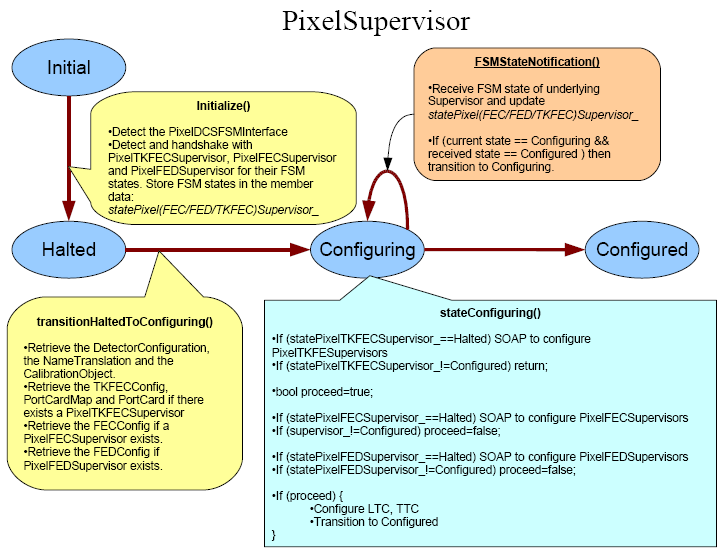
\includegraphics[width=160mm]{PixelSupervisorDAQDCS.png}
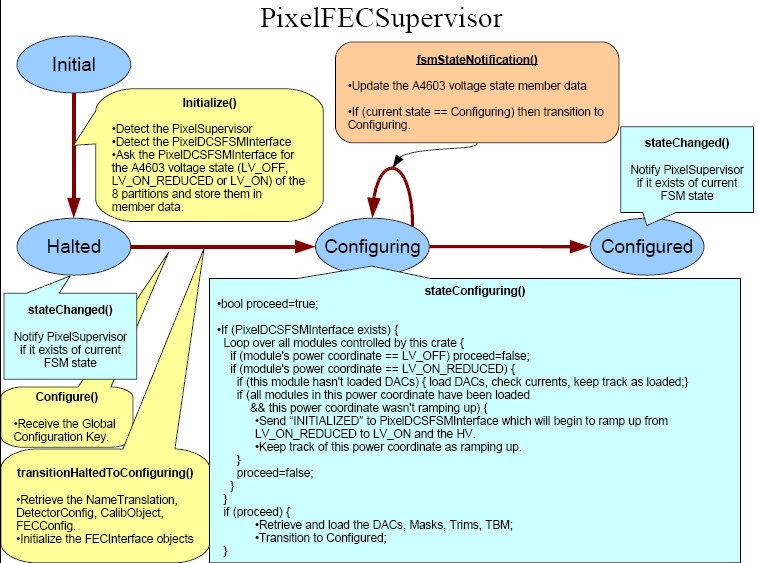
\includegraphics[width=160mm]{PixelFECSupervisorDAQDCS.png}
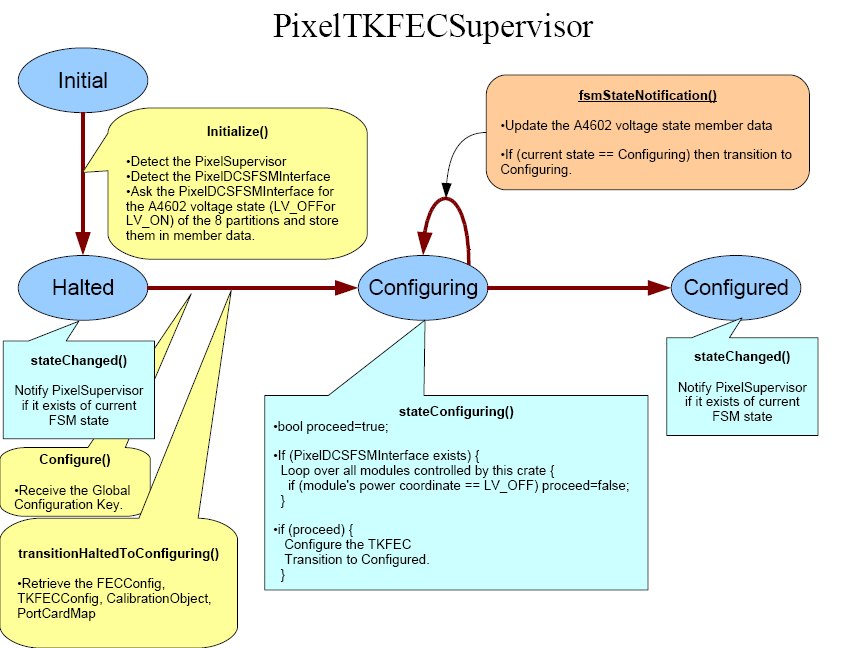
\includegraphics[width=160mm]{PixelTKFECSupervisorDAQDCS.png}
\end{center}

\begin{enumerate}
\item PixelFECSupervisor(s) and PixelTKFECSupervisor are initially 
      in their "Initial" state and await the "Initialize" command.

\item On receiving the "Initialize" command, PixelFECSupervisor(s) and 
      PixelTKFECSupervisor independently query PixelDCSFSMInterface.% with 
%%%%i think this is too much detail
%      the SOAP messages:
%      \begin{verbatim}
%<fsmStateRequest name="PixelFECSupervisor" type="PxlFEC" instance="1">
%</fsmStateRequest>
%
%<fsmStateRequest name="PixelTKFECSupervisor" type="TrkFEC" instance="1">
%</fsmStateRequest>
%      \end{verbatim}
%
%respectively.

\item The PixelDCSFSMInterface responds with information regarding 
      the voltage states.% with a SOAP message of the form:
%      \begin{verbatim}
%<fsmStateResponse>
%  <state partition="FPix_BmI">LV_ON;HV_ON</state>
%  <state partition="BPix_BpO">LV_ON;HV_OFF</state>
%  ...
%</fsmStateResponse>
%      \end{verbatim}

Note that in practice, the correct power state is never reported in
the ``Initialize'' step, because at P5 the ``Initialize'' transition
is always triggered immediately after starting the software, at which
point the PixelDCSFSMInterface has not yet had time to make
connections with the PSX server and be notified of the state of the
power supplies. Once the PSX server connections are made,
the correct power state is sent via the standard asynchronous
mechanism.


\item The PixelFECSupervisor(s) and PixelTKFECSupervisor update 
      their tri- and bi-state member data (for LV and HV as appropriate)
      according to the response from PixelDCSFSMInterface. This 
      concludes the "Initializing" transition
      and both the PixelFECSupervisor(s) and PixelTKFECSupervisors 
      land in their "Halted" states.

\item On receiving the "Configure" command, PixelFECSupervisor(s) 
      and PixelTKFECSupervisor
      check the status of their member data. If the appropriate 
      voltages are set then they go ahead
      with step \ref{item:FECconfig}. If the LV\_OFF state is found, configuration does not proceed.

\item \label{item:FECconfig}
If the PixelFECSupervisor finds that the LV is in state
LV\_ON\_REDUCED, the ROCs' DAC settings are loaded and programmed to
the ROCs. (It has been proposed to query the low-voltage currents
before and after this loading of DAC settings, in order to ensure that
the currents change when the DAC settings are loaded. However this
check is not implemented at present.) If the LV is already in state
LV\_ON (as is the case for the BPix, or on subsequent configurations
of the FPix), this step is skipped.

\item PixelFECSupervisor sends a SOAP message to PixelDCSFSMInterface to notify it that the FPix DAC settings have been loaded. The PixelDCSFSMInterface forwards this message to DCS via the PSX server.
%      The PixelDCSFSMInterface responds back with the raised values of the Digital Voltages.
%      PixelFECSupervisor resets its
%      tristate member data if this went fine or else 
%      transitions to its "Error" state.

%\begin{verbatim}
%<fsmStateNotification>
%  <state partition="FPix_BmI">INITIALIZED</state>
%  <state partition="BPix_BpO">INITIALIZED</state>
%</fsmStateNotification>
%\end{verbatim}

\item PixelFECSupervisors wait for an LV\_ON SOAP message from PixelDCSFSMInterface.

\item PixelFECSupervisors load their ROCs' DAC, mask and trim settings. When
programming the DACs, we check the state of the data member containing
the HV status.  The PixelTKFECSupervisors load the slow I2C
settings for CCU boards, Port Cards etc.

\item The PixelFECSupervisor(s) and PixelTKFECSupervisor(s) land in 
      their "Configured" state.

\end{enumerate}

During the configure step in PixelFECSupervisor, we follow the
``HV-dependent'' DAC programming procedure if and only if we are
configuring for a calibration. If we are configuring for Physics
running, then the ROCs are always disabled (treated as if the HV was
off).

\subsection{HV-dependent DAC programming}

At Configure (for calibrations only), and at the Start and Resume
transitions, we check the data members that store the HV status, and
we check the data members that track whether the ROCs were most
recently enabled or disabled. If we find that the HV is on and the
ROCs were previously disabled, we enable the ROCs. If we find that the
HV is off and the ROCs were previously enabled, then we disable the
ROCs. If we HV is on but the ROCs are already enabled, then we do
nothing; similarly if the HV is off but the ROCs are already disabled.

To disable the ROCs, we overwrite the VcThr DAC setting with 0
(high threshold), then disable the ROCs using the ROC control
register. These procedures are implemented in the PixelDACSettings
class. This class caches the DAC settings from the DB, and if we
override the VcThr setting with zero we do not change what is in the
cache, so no new DB accesses are needed when we want to enable the ROCs. The
PixelDACSettings::generateConfiguration() method has an argument for
the calling function in PixelFECSupervisor to indicate the status of
the HV. To enable the ROCs, the nominal VcThr and CCR settings are programmed.

%comment from Anders:
%For the PixelFECSupervisor to read out the current I suggest that 
%this is done by calling the PixelSupervisor. The PixelSupervisor
%will have all the configuration information needed to read the
%currents.

\subsection{Start and Resume transitions}
The status of the HV is checked and the DACs are programmed if needed, as explained above.

\subsection{Pause, Stop, and Halt transitions}
The ROCs are disabled as if the HV was off.


\subsection{Expected behavior}
As currently implemented, the following is the expected sequence of events when turning on the FPix:
\begin{itemize}
\item User turns FPix to ON in DCS
\item FPix is powered to LV\_ON\_REDUCED (called DIGITAL\_ON\_REDUCED in DCS)
\item User begins the Configure transition in PixelSupervisor
\item FPix DACs are programmed
\item POS notifies DCS that the DACs are programmed; POS then waits in the ``Configuring'' state
\item DCS raises the digital voltage to the nominal value
\item POS is notified that we have reached the LV\_ON state
\item DCS begins to ramp the high voltage.
\item Configuration in POS proceeds with the reprogramming of the DACs and the programming of the trims and masks
\item Configuration in POS finishes. At some point (probably after the end of configuration), the high voltage reaches its nominal value and DCS notifies POS that we have reached the HV\_ON state (called simply ON in DCS).
\item Because the HV was not on at the time of configuration, the DACs are set to the special settings used for HV\_OFF
\item User presses Start to begin a calibration in POS
\item The FEC Supervisor notices that the state of the HV has changed since the configuration. Therefore the VcThr and chip control register DACs are set to their nominal values. Because of this settings change, the user will see a large change in the amount of digital current drawn by the FPix.
\item The calibration proceeds as normal.
\end{itemize}

\subsection{Notes on hardcoding of information} \label{sec:dcshardcode}

Because the xdaq software (POS) and DCS use different naming schemes
and different granularity, several translations must be made in order
for POS to communicate with DCS. Some of these translations are
encoded in the {\tt interface.xml} file, while others are hard-coded
in the logic of the PixelDCSFSMInterface.

Specifically, the xml file defines which ROGs\footnote{readout
groups} exist, and which PVSS datapoint name belongs to which
ROG\footnote{These datapoints are used to indicate when POS has
configured the ROCs on a ROG.}. The xml file also defines the POS
applications that need to be notified in case the state of a ROG
changes.

The hardcoded logic in PixelDCSFSMInterface defines which ROG
correponds to which pieces of the detector (which ROCs are supplied by
which power supply).

In principle, this information could be instead contained in a database table with roughly 5 fields:


\begin{tabular}{ll}
Field in database & Example value \\
\hline
POS name          & FPix\_BmI\_D2\_BLD1 \\
DCS name          & {\tiny CMS\_TRACKER:PixelEndCap:PixelEndCap\_BmI:PixelEndCap\_BmI\_D2:PixelEndCap\_BmI\_D2\_ROG1} \\
datapoint name    & {\tiny cms\_trk\_dcs\_10:tkPg\_CAEN \textbackslash CMS\_TRACKER\_SY1527\_5 \textbackslash branchController05 \textbackslash easyCrate3 \ldots} \\
%{\tiny cms\_trk\_dcs\_10:tkPg\_CAEN \textbackslash CMS\_TRACKER\_SY1527\_5 \textbackslash branchController05 \textbackslash easyCrate3 \textbackslash easyBoard04.pixelSequence.configured} \\
SOAP connection (TKFEC) & PixelTKFECSupervisor instance 2 \\
SOAP connection (FEC) & PixelFECSupervisor instance 2 \\
\hline
\end{tabular}


With a table such as this, we could eliminate both the xml file and the hardcoding.

